%File: formatting-instruction.tex
\documentclass[letterpaper]{article}
\usepackage{flairs}

% REMOVE BEFORE SUBMITTING:
% \usepackage{lineno}
% \linenumbers

% JOURNAL VERSION TODO:
% Prove completeness
% Try to generalize proofs for other activation functions
% Figure out formal relationship between [\varphi^+] and other modalities (closure of [\varphi^+] might be public announcement?)
% Consider how we can view this in light of the energy function understanding of Hopfield nets (is there a property in our logic that expresses this?  could we express this with the kleene star/closure of [\varphi^+]?)

\usepackage{times}
\usepackage{helvet}
\usepackage{courier}
\usepackage{amssymb,amsthm,amsmath}
\usepackage{lscape}
\usepackage{bigstrut}
%\usepackage{MnSymbol}
\usepackage{bbm}
\usepackage{proof}
\usepackage{bussproofs}
\usepackage{lingmacros}
\usepackage{microtype}
\usepackage{setspace}
\usepackage{float}
\usepackage{mathtools}
\usepackage{tikz}
\usetikzlibrary{positioning,calc,arrows.meta,shapes.geometric,fit}
% INCOMPATIBLE (and completely changes the geometry of the page)
%\usepackage{fullpage}
\usepackage{pifont}
\newcommand{\cmark}{\ding{51}}%
\newcommand{\xmark}{\ding{55}}%

\usepackage{paralist}
\usepackage{enumitem}
\usepackage{etoolbox}
\AtBeginEnvironment{quote}{\par\singlespacing\small}

% INCOMPATIBLE WITH FLAIRS;
% but include with ArXiV version
% \usepackage{hyperref}
% \hypersetup{
%     colorlinks=true,
%     linkcolor=black,
%     urlcolor=blue,
%     citecolor=black,
% }
% \urlstyle{same}

\frenchspacing
\setlength{\pdfpagewidth}{8.5in}
\setlength{\pdfpageheight}{11in}
\pdfinfo{
/Title (The Logic of Hebbian Learning)
/Author (Caleb Kisby, Sa\'{u}l A. Blanco, Lawrence S. Moss)
/Keywords (Neurosymbolic AI, Hebbian Learning,
Dynamic Logics, Knowledge Representation and Reasoning, Nonmonotonic Reasoning, Preference Upgrade)}
\setcounter{secnumdepth}{0}

% Helpful spacing command
\newcommand{\compactcenter}[1]{\setlength{\abovedisplayskip}{0pt}{\[ #1 \]}}
\newcommand{\compactinline}[1]{\setlength{\abovedisplayskip}{2pt}{\setlength{\belowdisplayskip}{2pt}{\[ #1 \]}}}

\newcommand{\existsgeq}{\mbox{\sf AtLeast}}
\newcommand{\Pol}{\mbox{\emph{Pol}}}
  \newcommand{\nonered}{\textcolor{red}{=}}
  \newcommand{\equalsred}{\nonered}
  \newcommand{\redstar}{\textcolor{red}{\star}}
    \newcommand{\dred}{\textcolor{red}{d}}
    \newcommand{\dmark}{\dred}
    \newcommand{\redflip}{\textcolor{red}{flip}}
        \newcommand{\flipdred}{\textcolor{red}{\mbox{\scriptsize \em flip}\ d}}
        \newcommand{\mdred}{\textcolor{blue}{m}\textcolor{red}{d}}
        \newcommand{\ndred}{\textcolor{blue}{n}\textcolor{red}{d}}
\newcommand{\arrowm}{\overset{\textcolor{blue}{m}}{\rightarrow} }
\newcommand{\arrown}{\overset{\textcolor{blue}{n}}{\rightarrow} }
\newcommand{\arrowmn}{\overset{\textcolor{blue}{mn}}{\longrightarrow} }
\newcommand{\arrowmonemtwo}{\overset{\textcolor{blue}{m_1 m_2}}{\longrightarrow} }
\newcommand{\bluen}{\textcolor{blue}{n}}
\newcommand{\bluem}{\textcolor{blue}{m}}
\newcommand{\bluemone}{\textcolor{blue}{m_1}}
\newcommand{\bluemtwo}{\textcolor{blue}{m_2}}
\newcommand{\blueminus}{\textcolor{blue}{-}}

\newcommand{\bluedot}{\textcolor{blue}{\cdot}}
\newcommand{\bluepm}{\textcolor{blue}{\pm}}
\newcommand{\blueplus}{\textcolor{blue}{+ }}
\newcommand{\translate}[1]{{#1}^{tr}}
\newcommand{\Caba}{\mbox{\sf Caba}} 
\newcommand{\Set}{\mbox{\sf Set}} 
\newcommand{\Pre}{\mbox{\sf Pre}} 
\newcommand{\wmarkpolarity}{\scriptsize{\mbox{\sf W}}}
\newcommand{\wmarkmarking}{\scriptsize{\mbox{\sf Mon}}}
\newcommand{\smark}{\scriptsize{\mbox{\sf S}}}
\newcommand{\bmark}{\scriptsize{\mbox{\sf B}}}
\newcommand{\mmark}{\scriptsize{\mbox{\sf M}}}
\newcommand{\jmark}{\scriptsize{\mbox{\sf J}}}
\newcommand{\kmark}{\scriptsize{\mbox{\sf K}}}
\newcommand{\tmark}{\scriptsize{\mbox{\sf T}}}
\newcommand{\greatermark}{\mbox{\tiny $>$}}
\newcommand{\lessermark}{\mbox{\tiny $<$}}
%%{\mbox{\ensuremath{>}}}
\newcommand{\true}{\top}
\newcommand{\false}{\bot}
\newcommand{\upred}{\textcolor{red}{\uparrow}}
\newcommand{\downred}{\textcolor{red}{\downarrow}}
\usepackage[all,cmtip]{xy}
\usepackage{enumitem}
\usepackage{multicol}
\theoremstyle{definition}
\newtheorem{definition}{Definition}
\newtheorem{theorem}{Theorem}
\newtheorem{lemma}[theorem]{Lemma}
\newtheorem{claim}{Claim}
\newtheorem{corollary}{Corollary}
%\newtheorem{theorem}{Theorem}
\newtheorem{proposition}{Proposition}
\newtheorem{example}{Example}
\newtheorem{remark}[theorem]{Remark}
\newcommand{\semantics}[1]{[\![\mbox{\em $ #1 $\/}]\!]}
\newcommand{\abovearrow}[1]{\rightarrow\hspace{-.14in}\raiseonebox{1.0ex}
{$\scriptscriptstyle{#1}$}\hspace{.13in}}
\newcommand{\toplus}{\abovearrow{r}}
\newcommand{\tominus}{\abovearrow{i}} 
\newcommand{\todestroy}{\abovearrow{d}}
\newcommand{\tom}{\abovearrow{m}}
\newcommand{\tomprime}{\abovearrow{m'}}
\newcommand{\A}{\textsf{App}}
\newcommand{\At}{\textsf{At}}
\newcommand{\Emb}{\textsf{Emb}}
\newcommand{\EE}{\mathbb{E}}
\newcommand{\DD}{\mathbb{D}}
\newcommand{\PP}{\mathbb{P}}
\newcommand{\QQ}{\mathbb{Q}}
\newcommand{\LL}{\mathbb{L}}
\newcommand{\MM}{\mathbb{M}}
\usepackage{verbatim}
\newcommand{\TT}{\mathcal{T}}
\newcommand{\Marking}{\mbox{Mar}}
\newcommand{\Markings}{\Marking}
\newcommand{\Mar}{\Marking}
\newcommand{\Model}{\mathcal{M}}
\newcommand{\Nodel}{\mathcal{N}}
\renewcommand{\SS}{\mathcal{S}}
\newcommand{\TTM}{\TT_{\Markings}}
\newcommand{\CC}{\mathbb{C}}
\newcommand{\erase}{\mbox{\textsf{erase}}}
\newcommand{\set}[1]{\{ #1 \}}
\newcommand{\arrowplus}{\overset{\blueplus}{\rightarrow} }
\newcommand{\arrowminus}{\overset{\blueminus}{\rightarrow} }
\newcommand{\arrowdot}{\overset{\bluedot}{\rightarrow} }
\newcommand{\arrowboth}{\overset{\bluepm}{\rightarrow} }
\newcommand{\arrowpm}{\arrowboth}
\newcommand{\arrowplusminus}{\arrowboth}
\newcommand{\arrowmone}{\overset{m_1}{\rightarrow} }
\newcommand{\arrowmtwo}{\overset{m_2}{\rightarrow} }
\newcommand{\arrowmthree}{\overset{m_3}{\rightarrow} }
\newcommand{\arrowmcomplex}{\overset{m_1 \orr m_2}{\longrightarrow} }
\newcommand{\arrowmproduct}{\overset{m_1 \cdot m_2}{\longrightarrow} }
\newcommand{\proves}{\vdash}
\newcommand{\Dual}{\mbox{\sc dual}}
\newcommand{\orr}{\vee}
\newcommand{\uar}{\uparrow}
\newcommand{\dar}{\downarrow}
\newcommand{\andd}{\wedge}
\newcommand{\bigandd}{\bigwedge}
\newcommand{\arrowmprime}{\overset{m'}{\rightarrow} }
\newcommand{\quadiff}{\quad \mbox{ iff } \quad}
\newcommand{\Con}{\mbox{\sf Con}}
\newcommand{\type}{\mbox{\sf type}}
\newcommand{\lang}{\mathcal{L}}
\newcommand{\necc}{\Typ}
\newcommand{\vocab}{\mathcal{V}}
\newcommand{\wocab}{\mathcal{W}}
\newcommand{\Types}{\mathcal{T}_\mathcal{M}}
\newcommand{\mon}{\mbox{\sf mon}}
\newcommand{\anti}{\mbox{\sf anti}}
\newcommand{\FF}{\mathcal{F}}
\newcommand{\rem}[1]{\relax}


\newcommand{\raiseone}{\mbox{raise}^1}
\newcommand{\raisetwo}{\mbox{raise}^2}
\newcommand{\wrapper}[1]{{#1}}
\newcommand{\sfa}{\wrapper{\mbox{\sf a}}}
\newcommand{\sfb}{\wrapper{\mbox{\sf b}}}
\newcommand{\sfv}{\wrapper{\mbox{\sf v}}}
\newcommand{\sfw}{\wrapper{\mbox{\sf w}}}
\newcommand{\sfx}{\wrapper{\mbox{\sf x}}}
\newcommand{\sfy}{\wrapper{\mbox{\sf y}}}
\newcommand{\sfz}{\wrapper{\mbox{\sf z}}}
  \newcommand{\sff}{\wrapper{\mbox{\sf f}}}
    \newcommand{\sft}{\wrapper{\mbox{\sf t}}}
      \newcommand{\sfc}{\wrapper{\mbox{\sf c}}}
      \newcommand{\sfu}{\wrapper{\mbox{\sf u}}}
            \newcommand{\sfs}{\wrapper{\mbox{\sf s}}}
  \newcommand{\sfg}{\wrapper{\mbox{\sf g}}}

% INCOMPATIBLE WITH FLAIRS
% \newcommand{\sfvomits}{\wrapper{\mbox{\sf vomits}}}
% \newlength{\mathfrwidth}
%   \setlength{\mathfrwidth}{\textwidth}
%   \addtolength{\mathfrwidth}{-2\fboxrule}
%   \addtolength{\mathfrwidth}{-2\fboxsep}
\newsavebox{\mathfrbox}
\newenvironment{mathframe}
    {\begin{lrbox}{\mathfrbox}\begin{minipage}{\mathfrwidth}\begin{center}}
    {\end{center}\end{minipage}\end{lrbox}\noindent\fbox{\usebox{\mathfrbox}}}
    \newenvironment{mathframenocenter}
    {\begin{lrbox}{\mathfrbox}\begin{minipage}{\mathfrwidth}}
    {\end{minipage}\end{lrbox}\noindent\fbox{\usebox{\mathfrbox}}} 
 \renewcommand{\hat}{\widehat}
 \newcommand{\nott}{\neg}
  \newcommand{\preorderO}{\mathbb{O}}
 \newcommand{\PreorderP}{\mathbb{P}}
  \newcommand{\preorderE}{\mathbb{E}}
\newcommand{\preorderP}{\mathbb{P}}
\newcommand{\preorderN}{\mathbb{N}}
\newcommand{\preorderQ}{\mathbb{Q}}
\newcommand{\preorderX}{\mathbb{X}}
\newcommand{\preorderA}{\mathbb{A}}
\newcommand{\preorderR}{\mathbb{R}}
\newcommand{\preorderOm}{\mathbb{O}^{\bluem}}
\newcommand{\preorderPm}{\mathbb{P}^{\bluem}}
\newcommand{\preorderQm}{\mathbb{Q}^{\bluem}}
\newcommand{\preorderOn}{\mathbb{O}^{\bluen}}
\newcommand{\preorderPn}{\mathbb{P}^{\bluen}}
\newcommand{\preorderQn}{\mathbb{Q}^{\bluen}}
 \newcommand{\PreorderPop}{\mathbb{P}^{\blueminus}}
  \newcommand{\preorderEop}{\mathbb{E}^{\blueminus}}
\newcommand{\preorderPop}{\mathbb{P}^{\blueminus}}
\newcommand{\preorderNop}{\mathbb{N}^{\blueminus}}
\newcommand{\preorderQop}{\mathbb{Q}^{\blueminus}}
\newcommand{\preorderXop}{\mathbb{X}^{\blueminus}}
\newcommand{\preorderAop}{\mathbb{A}^{\blueminus}}
\newcommand{\preorderRop}{\mathbb{R}^{\blueminus}}
 \newcommand{\PreorderPflat}{\mathbb{P}^{\flat}}
  \newcommand{\preorderEflat}{\mathbb{E}^{\flat}}
\newcommand{\preorderPflat}{\mathbb{P}^{\flat}}
\newcommand{\preorderNflat}{\mathbb{N}^{\flat}}
\newcommand{\preorderQflat}{\mathbb{Q}^{\flat}}
\newcommand{\preorderXflat}{\mathbb{X}^{\flat}}
\newcommand{\preorderAflat}{\mathbb{A}^{\flat}}
\newcommand{\preorderRflat}{\mathbb{R}^{\flat}}
\newcommand{\pstar}{\preorderBool^{\preorderBool^{E}}}
\newcommand{\pstarplus}{(\pstar)^{\blueplus}}
\newcommand{\pstarminus}{(\pstar)^{\blueminus}}
\newcommand{\pstarm}{(\pstar)^{\bluem}}
\newcommand{\Reals}{\preorderR}
\newcommand{\preorderS}{\mathbb{S}}
\newcommand{\preorderBool}{\mathbbm{2}}
 \renewcommand{\o}{\cdot}
 \newcommand{\NP}{\mbox{\sc np}}
 \newcommand{\NPplus}{\NP^{\blueplus}}
  \newcommand{\NPminus}{\NP^{\blueminus}}
   \newcommand{\NPplain}{\NP}
    \newcommand{\npplus}{np^{\blueplus}}
  \newcommand{\npminus}{np^{\blueminus}}
   \newcommand{\npplain}{np}
   \newcommand{\np}{np}
   \newcommand{\Term}{\mbox{\sc t}}
  \newcommand{\N}{\mbox{\sc n}}
   \newcommand{\X}{\mbox{\sc x}}
      \newcommand{\Y}{\mbox{\sc y}}
            \newcommand{\V}{\mbox{\sc v}}
    \newcommand{\Nbar}{\overline{\mbox{\sc n}}}
    \newcommand{\Pow}{\mathcal{P}}
    \newcommand{\powcontravariant}{\mathcal{Q}}
    \newcommand{\Id}{\mbox{Id}}
    \newcommand{\pow}{\Pow}
   \newcommand{\Sent}{\mbox{\sc s}}
   \newcommand{\lookright}{\slash}
   \newcommand{\lookleft}{\backslash}
   \newcommand{\dettype}{(e \to t)\arrowminus ((e\to t)\arrowplus t)}
\newcommand{\ntype}{e \to t}
\newcommand{\etttype}{(e\to t)\arrowplus t}
\newcommand{\nptype}{(e\to t)\arrowplus t}
\newcommand{\verbtype}{TV}
\newcommand{\who}{\infer{(\nptype)\arrowplus ((\ntype)\arrowplus (\ntype))}{\mbox{who}}}
\newcommand{\iverbtype}{IV}
\newcommand{\Nprop}{\N_{\mbox{prop}}}
\newcommand{\VP}{{\mbox{\sc vp}}}
\newcommand{\CN}{{\mbox{\sc cn}}}
\newcommand{\Vintrans}{\mbox{\sc iv}}
\newcommand{\Vtrans}{\mbox{\sc tv}}
\newcommand{\Num}{\mbox{\sc num}}
%\newcommand{\S}{\mathbb{A}}
\newcommand{\Det}{\mbox{\sc det}}
\newcommand{\preorderB}{\mathbb{B}}
\newcommand{\simA}{\sim_A}
\newcommand{\simB}{\sim_B}
\newcommand{\polarizedtype}{\mbox{\sf poltype}}


\newcommand{\Typ}{\textrm{\textup{\textbf{T}}}}
\newcommand{\Prop}{\textsf{Prop}}
\newcommand{\Update}{\textsf{Update}}
\newcommand{\Inc}{\textsf{Inc}}
\newcommand{\AllNets}{\mathsf{Net}}
\newcommand{\Net}{\mathcal{N}}

\newcommand{\axiom}{\textsc}

\newcommand*{\bigchi}{\mbox{\Large$\chi$}}% big chi

\usepackage{xcolor}
\definecolor{myblue1}{RGB}{158,202,225}
\definecolor{myblue2}{RGB}{49,130,189}

% FIGURE SKIPS
% \setlength{\textfloatsep}{10pt}
% \setlength{\abovecaptionskip}{5pt}
% floatsep, textfloatsep, abovecaptionskip, belowcaptionskip

 \begin{document}
% This file is an adoption of the style file for AAAI Press 
% proceedings, working notes, and technical reports.  This file is made 
% with minimal changes by explicit permission from AAAI.
%
\title{The Logic of Hebbian Learning}

% \author{\#162 Author 1 \and \#162 Author 2\\
% Relevant Department, Institution, Location, Country\\
% \{email1, email2\}@institution\\
% \AND \#162 Author 3 \\
% Other Relevant Department, Institution, Location, Country\\
% email3@institution}

\author{Caleb Kisby \and Sa\'{u}l A. Blanco\\
Department of Computer Science, Indiana University, Bloomington, IN 47408, USA\\
\{cckisby, sblancor\}@indiana.edu
\AND Lawrence S. Moss \\
Department of Mathematics, Indiana University, Bloomington, IN 47405, USA\\
lmoss@indiana.edu}

\maketitle
\begin{abstract}
We present the logic of Hebbian learning, a dynamic logic whose semantics\footnote{A Python implementation of our semantics, using Tensorflow \& Keras \cite{tensorflow2015-whitepaper}), is available at
\textrm{https://github.com/ais-climber/neural-semantics}
% SAVE FOR JOURNAL VERSION
% (INCOMPATIBLE WITH FLAIRS)
% \href{https://github.com/ais-climber/neural-semantics}{https://github.com/ais-climber/neural-semantics}.
}
are expressed in terms of a layered neural network learning via Hebb's associative learning rule.  Its language consists of modality $\Typ \varphi$ (read ``typically $\varphi$,'' formalized as forward propagation), conditionals $\varphi \Rightarrow \psi$ (read ``typically $\varphi$ are $\psi$''), as well as dynamic modalities $[\varphi^+] \psi$ (read ``evaluate $\psi$ after performing Hebbian update on $\varphi$'').  We give axioms and inference rules that are sound with respect to the neural semantics; these axioms characterize Hebbian learning and its interaction with propagation.  The upshot is that this logic describes a neuro-symbolic agent that both learns from experience and also reasons about what it has learned.
\end{abstract}

%%%%%%%%%%%%%%%%%%%%%%%%%%%%%%%%%%%%%%%%%%%%
\section{Introduction}

Artificial intelligence  has  long  been  marked  by  a  schism between two of its major paradigms: symbolic reasoning and connectionist learning.  Neural systems have had wild success with learning from unstructured data, whereas symbolic reasoners are notorious for their rigidity.  On the other hand, symbolic systems excel at sophisticated (static) reasoning tasks that neural systems cannot readily learn.  Symbolic systems also tend to have more explainable reasoning, thanks to their use of explicit inferences in an intuitive language.  Moreover, due to their connection with logic, it is straightforward to compare the relative power and complexity of different symbolic reasoners.

% .\\
% \textbf{Symbolic Systems}
% \begin{compactitem}
%  \item[\textcolor{green}{\cmark}] Sophisticated rich reasoning
%  \item[\textcolor{green}{\cmark}] Explainable decisions
%  \item[\textcolor{red}{\xmark}] Notoriously rigid and static
%  \item[\textcolor{red}{\xmark}] Manual knowledge-engineering
% \end{compactitem}
% .\\
% \textbf{Neural Networks}
% \begin{compactitem}
%  \item[\textcolor{red}{\xmark}] Can't readily learn rich inference
%  \item[\textcolor{red}{\xmark}] ``Black Box'' decisions 
%  \item[\textcolor{green}{\cmark}] Learns from experience
%  \item[\textcolor{green}{\cmark}] Uses unstructured data
% \end{compactitem}

But as Valiant famously put it, intelligent cognitive agents must have \emph{both} ``the ability to learn from experience, and the ability to reason from what has been learned'' \cite{valiant2003three}.  \emph{Neuro-symbolic artificial intelligence} has emerged in the last few decades to address this challenge --- a monumental effort to integrate neural and symbolic systems, while retaining the advantages of both (see \cite{bader2005dimensions} and \cite{sarker2021neuro}, two surveys that span the decades).  Despite the cornucopia of neuro-symbolic proposals, the field has not yet agreed on an interface between the two that satisfyingly preserves both flexible learning and expressive reasoning.

Following the path set out by \cite{balkenius1991nonmonotonic} and \cite{leitgeb2001nonmonotonic,leitgeb2003nonmonotonic}, we advance the following proposal for the neuro-symbolic interface.  Rather than viewing the neural and symbolic as two different systems to be combined, we view them as two ways of interpreting the same agent.  More precisely, we view the dynamics of neural networks as the semantics to a formal logic.  This logic serves as a bridge between the neural network model and formal inference.

Previous work, particularly \cite{leitgeb2001nonmonotonic}, has considered how forward propagation in binary feed-forward nets forms a sound and complete semantics for the (static) conditional logic \textbf{CL} (\emph{loop-cumulative}).  The novelty of our paper is that we extend this logic by viewing a simple learning policy --- Hebbian update (``neurons that fire together wire together'') --- as a dynamic modality.  By doing so, we demonstrate that the dynamics of Hebbian learning (in binary feed-forward nets) directly corresponds to a particular dynamic multimodal logic that we call \emph{the logic of Hebbian learning}.
This logic meets Valiant's challenge:  It characterizes a cognitive agent that can learn from experience and also reason about what it has learned.

Our main result is the soundness of axioms and inference rules that characterize Hebbian learning.  The most interesting axioms involve the interaction between Hebbian update and forward propagation.  We also demonstrate how our logic models the learning of a concrete neural network. And although we leave the question of completeness open, we close by considering the importance of completeness for logics of this kind.

%%%%%%%%%%%%%%%%%%%%%%%%%%%%%%%%%%%%%%%%%%%%
\section{Related Work}

\subsubsection{Logics with Neural Semantics.}
The idea that we can view neural networks as the semantics for symbolic reasoning dates back to \cite{mcculloch1943logical}.  Our work builds on a recent reimagining of this \`a la \cite{balkenius1991nonmonotonic}, \cite{leitgeb2001nonmonotonic,leitgeb2003nonmonotonic,leitgeb2018neural}, which formally characterize the dynamics of inhibitory neural networks as conditional logics.  Similarly, \cite{blutner2004nonmonotonic} demonstrates that Hopfield networks correspond to the logic of what he calls ``weight-annotated Poole systems.''  More recently, \cite{giordano2021} describe multilayer perceptrons and self-organizing maps in terms of typicality in defeasible description logics.  Yet no neural semantics to date has tackled the issue of learning --- doing this for Hebbian learning is precisely the contribution of our paper.

\subsubsection{Neuro-Symbolic AI.}
Across the neuro-symbolic literature, an ubiquitous premise is that integration involves combining or composing otherwise distinct neural and symbolic modules.  In contrast, this paper presents the neural and symbolic as two perspectives we can have about the same agent.

To our knowledge, the combined work of \cite{garcez2001symbolic} and \cite{garcez2008neural} is the only neuro-symbolic proposal (besides neural semantics, see above) that exhibits this intimate interface between the two.  The former gives a formally sound method for extracting conditionals from a network and the latter gives a method for build neural network models from rules (in a variety of different logics).  When combined, we can freely translate between a neural network and its beliefs.  But unlike our work, this framework does not offer a logical account of the neural network's learning.

% SAVE FOR JOURNAL VERSION
%Consider Henry Kautz' recent taxonomy of neuro-symbolic systems \cite{kautz-2020future}: All five of his categories involve combining or composing otherwise distinct neural and symbolic modules.

\subsubsection{Dynamic Logics for Learning.}
Two recent papers, \cite{baltag2019dynamic} and \cite{baltag2019right}, also present dynamic multimodal logics that characterize learning.  The former models an individual's learning in the limit, whereas the latter models supervised learning as a game played between student and teacher.  But it is unclear how learning policies expressed in these logics might relate to specific neural implementations of learning such as Hebbian update and backpropagation.

Furthermore, the syntax and inferences of our logic do not resemble either of these in a meaningful way. Perhaps the closest logics to ours are dynamic logics of \emph{preference upgrade}, in the sense of \cite{van2007prefupgrade}.  In particular, consider the modalities $[{\Uparrow} \varphi]$ (lexicographic upgrade) and $[{\uparrow} \varphi]$ (elite change) \cite{van2007beliefrevision}.  Both of these operators implement policies for modifying an agent's preference relation $<$ over possible worlds.  As with our logic, the key axioms characterizing these policies deal with their interaction with conditionals $\varphi \Rightarrow \psi$.  But the semantics of our logic have a different flavor; we leave the issue of how our neural semantics relate to classical preference relations to future work.  In addition, both $[{\Uparrow} \varphi]$ and $[{\uparrow} \varphi]$ are reducible to the static language of conditionals, whereas it is presently unclear how our $[\varphi^+]$ might reduce to its base language.


%%%%%%%%%%%%%%%%%%%%%%%%%%%%%%%%%%%%%%%%%%%%
\section{Background}

\subsection{Neural Network Models}

A model of the logic of Hebbian learning is just a special type of artificial neural network that we call a \emph{binary feedforward neural network} (BFNN).

% \textbf{Neural networks} are given by ${\Net = \langle N, E, W, A, O, \eta \rangle}$:
% \[\arraycolsep=2.5pt
% \begin{array}{ll|ll}
% N & \mbox{Set of neurons} & 
% W: N \times N & \mbox{Weights}\\

% E & \mbox{Excitatory connections} & 
% A^{(n)} : \mathbb{R}^k \to \mathbb{R} & \mbox{Activation function}\\

% \eta \in \mathbb{R} & \mbox{Learning rate} &
% O^{(n)} : \mathbb{R} {\to} \set{0, 1} & \mbox{Output function}
% \end{array}
% \]
% \begin{compactitem}
% \item \textbf{Feedforward:} $E$ has no cycles with all nonzero weights
% \item \textbf{Binary:} $O^{(n)}(x) \in \set{0, 1}$
% \item \textbf{Monotonic:} $A^{(n)}(\vec{x})$ is monotonically increasing\\ (this includes sigmoid functions)
% \end{compactitem}

\begin{definition} A BFNN is a pointed directed graph ${\Net = \langle N, E, W, A, O, \eta \rangle}$, where
\begin{itemize}
    \item $N$ is a finite nonempty set (the set of neurons)
    \item $E \subseteq N \times N$ (the set of excitatory connections)
    \item $W : N \times N \to \mathbb{R}$ (the weight of a given connection)
    \item $A$ is a function which maps each $n \in N$ to
    $A^{(n)} : \mathbb{R}^k \to \mathbb{R}$ (the activation function for $n$, where $k$ is the indegree of $n$)
    \item $O$ is a function which maps each $n \in N$ to 
    $O^{(n)} : \mathbb{R} \to \set{0, 1}$ (the output function for $n$)
    \item $\eta \in \mathbb{R}, \eta \geq 0$ (the learning rate)
\end{itemize}
Moreover, BFNNs are \emph{feed-forward}, i.e. they do not contain cycles of edges with all nonzero weights.  BFNNs are also \emph{binary}, i.e. the output of each neuron is in $\set{0, 1}$.  This binary assumption is unrealistic in practice, although letting it go is just a matter of extending our two-valued logic towards a fuzzy-valued logic (left to future work).

We further require that each composition of activation and output functions ${O^{(n)} \circ A^{(n)}}$ is \textit{strictly} monotonically increasing, i.e. for all $\vec{x}, \vec{y} \in \mathbb{R}^k$,
\[
\mbox{If } \vec{x} < \vec{y} \mbox{ then } O^{(n)}(A^{(n)}(\vec{x})) < O^{(n)}(A^{(n)}(\vec{y}))
\]
Our activation functions include in particular those sigmoid functions commonly used for neural networks in practice.
\end{definition}

We write $W_{ij}$ to mean $W(i,j)$, for ${(i, j) \in E}$.  When $m_i$ is drawn from a sequence ${m_1, \ldots, m_k}$, we write ${A^{(n)}(\smash{\overrightarrow{W}}(m_i, n))}$ as shorthand instead of the full expression $A^{(n)}(W(m_1, n), \ldots, W(m_k, n))$.


\subsection{The Dynamics of Propagation}

Of course, BFNNs are not merely static directed graphs, but are dynamic in nature.  When a BFNN receives a signal (which we model as the initial state), it propagates that signal forward until the state of the net stabilizes.  This stable state of the net is considered to contain the net's response (answer) to the given signal (question).  We model forward propagation as follows, drawing heavily from the approach proposed by \cite{leitgeb2001nonmonotonic}.\footnote{Note that \cite{leitgeb2001nonmonotonic} defines propagation for \emph{inhibition nets}, i.e. weightless BFNNs with both excitatory and inhibitory connections.  But this paper also proves that inhibition nets and BFNNs are equivalent with respect to their propagation structure.   So we import the ideas and results here.}  

We consider a neuron $n$ active if its activation $A^{(n)}$ triggers an output $O^{(n)}$ of $1$ (intuitively, if the neuron fires).  Since our BFNNs are binary, either a given neuron is active ($1$) or it is not ($0$).  So we can identify the state of $\Net$ with the set of neurons that are active.  For a given BFNN $\Net$, let its set of states be
\[
    \Set = \set{S \mid S \subseteq N}
\]

Neurons in a state $S \in \Set$ can subsequently activate new neurons, which activate yet more neurons, until eventually the state of $\Net$ stablizes.  We call this final state of affairs $\Prop(S)$, the \emph{propagation} of $S$.

\begin{definition}
Let $\Prop : \Set \to \Set$ be defined recursively as follows:  $n \in \Prop(S)$ iff either
\begin{itemize}
    \item[] \textbf{(Base Case)} $n \in S$, or
    \item[] \textbf{(Constructor)} For those $m_1, \ldots, m_k \in \Prop(S)$ such that $(m_i, n) \in E$ we have
    \[
    O^{(n)}(A^{(n)}(\smash{\overrightarrow{W}}(m_i, n))) = 1
    \]
\end{itemize}
\end{definition}

% INCLUDE IN JOURNAL VERSION:
% (not extremely relevant here, unless I have more to say about it...)
Alternatively, consider a finite automaton with state space $\Set$ and transition function $F_{S^\ast} : \Set \to \Set$ tracking the propagation of an initial state $S^\ast$ through $\Net$.  We can view $\Prop(S^\ast)$ as a fixed point of $F_{S^\ast}$ \cite{leitgeb2001nonmonotonic}.
% Leitgeb claims that Prop(S*) is *the unique* fixed point.  I'd like to be able to say this, but I should prove it myself for BFNNs.

The key insight of \cite{leitgeb2001nonmonotonic} is that we can neatly characterize the algebraic structure of $\Prop$ as a closure operator.

\begin{theorem}
Let $\Net \in \AllNets$.  For all $S, S_1, S_2 \in \Set$,
%$\Prop$ satisfies
\begin{itemize}
    \item \textbf{(Inclusion)} $S \subseteq \Prop(S)$
    
    \item \textbf{(Idempotence)} $\Prop(S) = \Prop(\Prop(S))$
    
    \item \textbf{(Cumulative)} If ${S_1 \subseteq S_2 \subseteq \Prop(S_1)}$\\ then ${\Prop(S_1) = \Prop(S_2)}$
    
    \item \textbf{(Loop)} If ${S_1 \subseteq \Prop(S_0)}, \ldots, {S_n \subseteq \Prop(S_{n-1})}$ and ${S_0 \subseteq \Prop(S_n)}$, then ${\Prop(S_i) = \Prop(S_j)}$\\
    for all $i, j \in \set{0, \ldots, n}$
\end{itemize}
\end{theorem}

Crucially, $\Prop$ is not monotonic --- it is not the case that for all $S_1, S_2 \in \Set$, if $S_1 \subseteq S_2$, then $\Prop(S_1) \subseteq \Prop(S_2)$.  The reason for this is that a BFNN's weights $W_{ij}$ can be negative, which allows $S_2$ to inhibit the activation of new neurons that were otherwise activated by $S_1$.  But in place of monotonicity, $\Prop$ is \emph{loop-cumulative} (in the terminology of \cite{kraus1990nonmonotonic}).

%%%%%%%%%%%%%%%%%%%%%%%%%%%%%%%%%%%%%%%%%%%%
\section{From Hebbian Learning to Logic}

%%%%%%%%%%%%%%%%%%%%%%%%%%%%%%%%%%%%%%%%%%%%
\subsection{The Dynamics of Hebbian Learning}

The plan from here is to extend this logic of propagation by providing an account of Hebbian learning.  Our goal is to cast Hebbian update as a dynamic modality, so that we can explore its interactions with $\Prop$ in symbolic language.  As with $\Prop$, we start by outlining the algebraic structure of Hebbian update.

Hebb's classic learning rule \cite{hebb-organization-of-behavior-1949} states that when two adjacent neurons are simultaneously and persistently active, the connection between them strengthens.  In contrast with, e.g. backpropagation, Hebbian learning is errorless and unsupervised.  Another key difference is that Hebbian update is local --- the change in a weight $\Delta W_{ij}$ depends only on the activation of the immediately adjacent neurons.  For this reason, the Hebbian family of learning policies has traditionally been considered more biologically plausible than backpropagation.  There are many variations of Hebbian learning, but we only consider the most basic (unstable, no weight decay) form of Hebb's rule:  $\Delta W_{ij} = \eta x_i x_j$, where $\eta$ is the learning rate and $x_i, x_j$ are the outputs of adjacent neurons $i$ and $j$, respectively.

In order to incorporate Hebb's rule into our framework, we introduce a function $\Inc$ (``increase the weights'') to strengthen those edges in a BFNN $\Net$ whose neurons are active when we feed $\Net$ a signal $S \in \Set$.  
% SAVE EXPOSITION FOR THE JOURNAL
% ALSO needs to be rephrased, technically incorrect
%We can get the output of a neuron $n$ via the following characteristic function.
\begin{definition}
For $S \in \Set$, let 
$\bigchi_S : N \to \set{0, 1}$ be given by $\bigchi_S(n) = 1$ iff $n \in S$
\end{definition}

% SAVE EXPOSITION FOR THE JOURNAL
% $\Inc$ can now be defined as follows.
\begin{definition}
Let ${\Inc : \AllNets \times \Set \to \AllNets}$ be given by $\Inc(\langle N, E, W, A, O, \eta \rangle, S) = \langle N, E, W^\ast, A, O, \eta \rangle$, where
\[
    W_{ij}^\ast = W_{ij} + \eta \cdot \bigchi_{\Prop(S)}(i) \cdot  \bigchi_{\Prop(S)}(j)
\]
\end{definition}
Notice that we propagate $S$ before getting the active status of neurons.  
This is because otherwise
%when a Hebbian net receives a signal $S$, it strengthens all connections that are activated by $S$.  
%Otherwise, 
we would never strengthen connections beyond the input layer.

We were able to formulate the algebraic properties of $\Prop$ in terms of $\Set$ containment.  Similarly, we express the properties of $\Inc$ in terms of $\AllNets$ containment.  
% SAVE EXPOSITION FOR JOURNAL VERSION
%We define the notion of \emph{subnet} ($\preceq$) as follows.

\begin{definition}
Let $\Net_1, \Net_2 \in \AllNets$ differ only in their weights.  We write
\[
    \Net_1 \preceq \Net_2
\]
to mean that for all $S \in \Set$, $\Prop_{\Net_1}(S) \subseteq \Prop_{\Net_2}(S)$.  We use $\cong$ to express that $\Net_1 \preceq \Net_2$ and $\Net_2 \preceq \Net_1$.
\end{definition}

For example, $\Inc(\Net, S)$ is a supernet of $\Net$ because strengthening weights via the $\Inc$ operation only has the potential to \emph{expand} future propagations.  To further cement this intuition, consider the least upper bound $\mathcal{N}^{lub}$ of $\preceq$.  $\mathcal{N}^{lub}$ is that net whose weights have been ``maximally'' strengthened, and so every propagation $\Prop(S)$ results in the entire set $N$.

We have the following test to determine if $\Net_1 \preceq \Net_2$.
\begin{lemma}
\label{lemma:subnet->leq}
Suppose $\Net_1$ and $\Net_2$ are the same except for their weights, and let $S \in \Set$.  Then ${\Prop_{\Net_1}(S) \subseteq \Prop_{\Net_2}(S)}$ iff for all $n \in \Prop_{\Net_1}(S)$ and for those $m_1, \ldots, m_k \in \Prop_{\Net_1}(S)$ such that $(m_i, n) \in E$,
\begin{equation}\tag{$\ast$}
\label{eqn:weight-condition}
  \begin{gathered}
    O^{(n)}(A^{(n)}(\smash{\overrightarrow{W}}_{\Net_1}(m_i, n))) = 1 \\
    \mbox{implies} \\
    O^{(n)}(A^{(n)}(\smash{\overrightarrow{W}}_{\Net_2}(m_i, n))) = 1
  \end{gathered}
\end{equation}
\end{lemma}

\begin{corollary}
\label{corollary:subnet->weights}
Let $\Net_1, \Net_2$ be the same except for their weights.  Then $\Net_1 \preceq \Net_2$ iff for all $n \in N$ and for those $m_1, \ldots, m_k \in N$ such that $(m_i, n) \in E$, (\ref{eqn:weight-condition}) holds.
\end{corollary}
Notice that the right-hand side of this biconditional does not mention $\Prop$; this test reduces the \emph{dynamic} condition ($\Net_1 \preceq \Net_2$) to a \emph{static} condition (a statement about the relative weights between $\Net_1$ and $\Net_2$).

These two facts are exactly what we need for the following algebraic characterization of $\Inc$.

\begin{theorem}
For all $\Net, \Net_1, \Net_2 \in \AllNets$ and $S, S_1, S_2 \in \Set$, $\Inc$ satisfies
\begin{itemize}
    \item \textbf{(Inclusion)}
    $\Net \preceq \Inc(\Net, S)$
    
    \item \textbf{(Absorption)}
    $\Inc(\Net, \Prop(S)) \cong \Inc(\Net, S)$
    
    \item \textbf{(Monotonicity in $\Net$)} if ${\Net_1 \preceq \Net_2}$ \\
    then ${\Inc(\Net_1, S) \preceq \Inc(\Net_2, S)}$
    
    % \item \textbf{(Distributivity over Complement)}
    % \setlength{\jot}{0pt}{
    % \setlength{\abovedisplayskip}{0pt}{
    % \begin{multline*}
    % \Prop_{\Inc(\Net, \overline{S_2})}(S_1) =\\ \Prop_{\Inc(\Net, S_2)}(\overline{S_1}) \cap \Prop_{\Net}(S_1)
    % \end{multline*}
    % }}
    
    \item \textbf{(Local)}
    \compactinline{
    \Prop_{\Inc(\Net, S_2)}(S_1) \subseteq \Prop_\Net(S_1) \cup \Prop_\Net(S_2)
    }
    
    \item \textbf{(Cumulative)} If ${\Prop_\Net(S_1) \subseteq \Prop_\Net(S_2)}$\\ and ${\Prop_\Net(S_2) \subseteq \Prop_{\Inc(\Net, S)}(S_1)}$,\\
    then $\Prop_{\Inc(\Net, S)}(S_1) = \Prop_{\Inc(\Net, S)}(S_2)$
    
    \item \textbf{(Loop)} If ${\Prop_\Net(S_1) \subseteq \Prop_{\Inc(\Net, S)}(S_0)}$,\\
    $\ldots, {\Prop_\Net(S_n) \subseteq \Prop_{\Inc(\Net, S)}(S_{n-1})}$,\\
    and 
    ${\Prop_\Net(S_0) \subseteq \Prop_{\Inc(\Net, S)}(S_n)}$,\\
    then ${\Prop_{\Inc(\Net, S)}(S_i) = \Prop_{\Inc(\Net, S)}(S_j)}$\\
    for all $i, j \in \set{0, \ldots, n}$
\end{itemize}
\label{thm:inc-props}
\end{theorem}

Like $\Prop$, $\Inc$ is loop-cumulative (in $S$).  But also like $\Prop$, $\Inc$ is not monotonic in $S$.  For a counterexample of $S$-monotonicity, see Figure~\ref{fig:full-example} (discussed in more detail towards the end of this paper).

%%%%%%%%%%%%%%%%%%%%%%%%%%%%%%%%%%%%%%%%%%%%
\subsection{Syntax and Semantics}

We can now introduce the logic of Hebbian learning.  Let $p, q, \ldots$ be finitely many propositional variables.  These represent fixed, `ontic' states, i.e. established choices of neurons that correspond to features in the external world.  For example, $p$ might be the set of neurons that encapsulates the color \emph{pink}.  We presume that we already agree on these states, although we acknowledge that this is a major unresolved empirical issue.  As for more complex formulas:

\begin{definition}  Formulas of our language $\lang$ are given by
\[
\varphi \Coloneqq p \mid \top \mid \neg \varphi \mid \varphi \land \varphi \mid \varphi \to \varphi \mid \varphi \Rightarrow \varphi \mid \Typ \varphi \mid [\varphi^+] \varphi
\]
where $p$ is any propositional variable.  We define $\bot$, $\lor$, $\leftrightarrow$, $\Leftrightarrow$, and their duals $\langle \Typ \rangle, \langle \varphi^+ \rangle$ in the usual way.
\end{definition}

The modalities $\Typ$ and $[\varphi^+]$ reflect our two operations $\Prop$ and $\Inc$, respectively.  We intend for $\Typ \varphi$ to denote ``the propagation of signal $\varphi$,'' and for $[\varphi^+] \psi$ to denote ``after performing Hebbian update on $\varphi$, evaluate $\psi$.''  We import ${\varphi \Rightarrow \psi}$ from \cite{leitgeb2001nonmonotonic}, read ``the propagation of signal $\varphi$ contains $\psi$''.  Note that ${\varphi \Rightarrow \psi}$ is redundant (equivalent to $\Typ \varphi \to \psi$ using the semantics below), though we keep it in our syntax because it conveniently expresses ``the net \emph{classifies} $\varphi$ as $\psi$'' (if $\varphi$ is interpreted as an input and $\psi$ as a classification).

Our formulas also have more classical alternative readings, divorced from the dynamics of neural networks.  Following \cite{leitgeb2001nonmonotonic}, we will define $\varphi \Rightarrow \psi$ such that it has the conditional reading ``typically $\varphi$ are $\psi$'' (where $\varphi$ and $\psi$ are read as generics, e.g. ``typically birds fly'').  This gives us a natural preferential reading for $\Typ \varphi$ as ``typically $\varphi$'' or ``the typical $\varphi$.''\footnote{Our notation takes inspiration from \cite{giordano2021}, which formalizes the dynamics of a net via a concept constructor $\Typ$ in the description logic $\mathcal{ALC}$.  Note the subtle difference between their typicality inclusions $\Typ(\varphi) \sqsubseteq \psi$ and our $\Typ \varphi \to \psi$: Ours flips the direction of containment.} 
Finally, Hebbian learning $[\varphi^+] \psi$ has a dual reading as \emph{preference upgrade}  \cite{van2007prefupgrade}.  As mentioned in the Related Work section, we leave the question concerning how $[\varphi^+]$ can be viewed classically as updating a preference relation to future work.

A model of our logic is just a BFNN $\Net$ equipped with an interpretation function $\semantics{\cdot} : \lang \to \Set_\Net$.

\begin{definition}
Let $\Net \in \AllNets$.  Our semantics are defined recursively as follows:
\begin{equation*}
\boxed{
\begin{array}{lcl}
\semantics{p} & & \in \Set \mbox{ is fixed, nonempty} \\
\semantics{\top} & = & \emptyset \\
\semantics{\neg \varphi} & = & \overline{\semantics{\varphi}}\\
\semantics{\varphi \land \psi} & = & \semantics{\varphi} \cup \semantics{\psi}\\
\semantics{\varphi \to \psi} & = & \semantics{\top} \textrm{ iff } \semantics{\varphi} \supseteq \semantics{\psi}{,} \textrm{ else } \semantics{\bot}\\
\semantics{\varphi \Rightarrow \psi} & = & \semantics{\top} \textrm{ iff } \Prop(\semantics{\varphi}) \supseteq \semantics{\psi}{,} \textrm{ else } \semantics{\bot}\\
\semantics{\Typ \varphi} & = & \Prop(\semantics{\varphi}) \\
\semantics{[\varphi^+] \psi} & = & \semantics{\psi}_{\Inc(\Net, \semantics{\varphi})} \\
\end{array}
}
\end{equation*}
\end{definition}

It may seem odd that we interpret $\land$ as union (instead of intersection), $\to$ as superset (instead of subset), and $\top$ as $\emptyset$ (instead of $N$).  But this choice reflects the intuition that neurons act as ``elementary-feature-detectors'' \cite{leitgeb2001nonmonotonic}.  
% possible thing to remove:
For example, say $\semantics{\varphi}$ represents those neurons that are \textit{necessary} for detecting an apple, and $\semantics{\psi}$ represents those neurons that are \textit{necessary} for detecting the color red. 
% add 'for instance,'
If the net observes a red apple ($\varphi \land \psi$), both the neurons detecting red-features $\semantics{\varphi}$ and the neurons detecting apple-features $\semantics{\psi}$ necessarily activate, i.e. $\semantics{\varphi} \cup \semantics{\psi}$ activates.  As for implication, ``every apple is red'' (${\varphi \to \psi}$) holds for a net iff whenever the neurons detecting apple-features $\semantics{\varphi}$ necessarily activate, so do the neurons detecting red-features $\semantics{\psi}$.  But this is only true if ${\semantics{\varphi} \supseteq \semantics{\psi}}$.  This justifies us reading propositional connectives classically, despite the backwards flavor of the semantics.\looseness=-1

% [implication] means that whenever a car is detected, the color yellow must be detected as well.  That is, the set of neurons detecting car-features $\semantics{\varphi}$ must \emph{contain} those neurons detecting yellow-features $\semantics{\psi}$.

Our interpretation of formulas is completely algebraic, in the sense that formulas denote sets rather than truth-values.  But we can consider formulas to have truth-values as follows.

\begin{definition}
$\Net \models \varphi$ iff $\semantics{\varphi}_\Net = \emptyset$.
\end{definition}

This choice also appears to be strange at its surface.  But it is a natural one in light of the fact that we defined $\semantics{\top} \coloneqq \emptyset$.  For example, consider implication: $\Net \models \varphi \to \psi$ holds iff $\semantics{\varphi \to \psi} = \emptyset = \semantics{\top}$, which holds iff $\semantics{\varphi} \supseteq \semantics{\psi}$ by our semantics.

A curious consequence is that if $\Net \models \varphi$ and $\varphi$ cannot be written to contain an implication $\to$, then $\varphi$ must be a tautology.  But we do not consider this troubling, since it only makes sense to consider a neural network's judgment of $\varphi$ when given a state $\semantics{\psi}$ the net is in.

%%%%%%%%%%%%%%%%%%%%%%%%%%%%%%%%%%%%%%%%%%%%
\subsection{Inference and Axioms}


\begin{figure}[ht!]
\begin{equation*}
\boxed{
\begin{array}{ll}
    & \textbf{Basic Axioms}\\
    
    \axiom{(PC)} & \mbox{All propositional tautologies}\\

    \axiom{(Dual)} & \langle \Typ \rangle \varphi \leftrightarrow \neg \Typ \neg \varphi\\
    
    \axiom{(N)} & \Typ \top\\
    
    \axiom{(T)} & \Typ \varphi \to \varphi\\
    
    \axiom{(4)} & \Typ \varphi \to \Typ \Typ \varphi\\
    
    & \textbf{Inference Rules}\\

    \axiom{(MP)} & \frac{\varphi \quad \varphi \to \psi}{\psi} \\
    
    \axiom{(Typ)} & \frac{\varphi \Rightarrow \psi}{\Typ \varphi \to \psi} \quad \frac{\Typ \varphi \to \psi}{\varphi \Rightarrow \psi} \\

    % Redundant given (N), and (N) is more often used for non-normal modal logics.
    % (\axiom{Nec}_\Typ) & \frac{\varphi}{\Typ \varphi} \\
    
    (\axiom{C}_\Rightarrow) & \frac{\varphi \to \psi \quad \psi \Rightarrow \varphi}{\varphi \Leftrightarrow \psi} \\
    
    (\axiom{Loop}_\Rightarrow) & 
    \frac{\varphi_0 \Rightarrow \varphi_1
    \cdots
    \varphi_{k-1} \Rightarrow \varphi_k \enskip
    \varphi_k \Rightarrow \varphi_0}
    {\varphi_0 \Rightarrow \varphi_k} \\
    
    (\axiom{Nec}_+) & \frac{\psi}{[\varphi^+] \psi} \\
    
    (\axiom{C}_+) & \frac{\psi \to \rho \quad [\varphi^+] \rho \to \psi}{[\varphi^+] \psi \leftrightarrow [\varphi^+] \rho} \\
    
    (\axiom{Loop}_+) & \frac{[\varphi^+] \psi_0 \to \psi_1 
    \cdots 
    [\varphi^+] \psi_{k-1} \to \psi_k \enskip 
    [\varphi^+] \psi_k \to \psi_0}
    {[\varphi^+] \psi_0 \to \psi_k} \\
    
    & \textbf{Reduction Axioms}\\

    (\axiom{R}_p) & [\varphi^+] p \leftrightarrow p \\
    
    (\axiom{R}_\neg) & [\varphi^+] \neg \psi \leftrightarrow \neg [\varphi^+] \psi \\
    
    (\axiom{R}_\land) & [\varphi^+] (\psi \land \rho) \leftrightarrow ([\varphi^+] \psi \land [\varphi^+] \rho)\\
    
    (\axiom{Nest}_\Typ) & [\Typ \varphi^+] \psi \leftrightarrow [\varphi^+] \psi \\
    
    & \textbf{Key Axioms}\\

    % Agent prefers the result of update in advance
    % "No Disappointment"
    \axiom{(NS)} & [\varphi^+] \Typ \psi \to \Typ [\varphi^+] \psi\\
    
    % "Preference Persistence"
    % (one of the four major effects under the umbrella of "confirmation bias"
    \axiom{(TP)} & \Typ [\varphi^+] \psi \land \Typ \varphi \to [\varphi^+] \Typ \psi\\
\end{array}
}
\end{equation*}
\caption{A list of sound rules and axioms of the logic of Hebbian learning.  We leave the question of completeness to future work.}
\label{fig:proof-system}
\end{figure}

The proof system for our logic is as follows.  We have $\proves \varphi$ iff either $\varphi$ is an axiom, or $\varphi$ follows from previously obtained formulas by one of the inference rules.  If $\Gamma \subseteq \lang$ is a set of formulas, we consider $\Gamma \proves \varphi$ to hold whenever there exist finitely many $\psi_1, \ldots, \psi_k \in \Gamma$ such that $\proves \psi_1 \land \ldots \land \psi_k \to \varphi$.

We list the axioms and inference rules for our logic in Figure~\ref{fig:proof-system}.  Our main result is the soundness of these axioms and rules --- we do not claim that this list forms a complete axiomatization (we revisit the question of completeness in the Conclusion).

The static base of our logic can either be viewed as the conditional logic \textbf{CL} (loop-cumulative), or alternatively as the modal logic characterized by $\Typ$ along with inference rules $(\axiom{C}_\Rightarrow), (\axiom{Loop}_\Rightarrow)$ expressing the loop-cumulativity of $\Prop$.  Linking these perspectives is the rule $(\axiom{Typ})$.  As a modality, $\Typ$ is neither normal, regular, nor monotonic, but it is classical.  Note for instance that the normal modal property \axiom{(K)} (expressed in terms of $\Typ$) is equivalent to
\[
\axiom{(K)} \quad \Typ (\varphi \land \psi) \leftrightarrow (\Typ \varphi \land \Typ \psi)
\]
neither direction of which is sound in our logic.

As with $\Typ$, we have the inference rules $(\axiom{Nec}_+)$, $(\axiom{C}_+)$, $(\axiom{Loop}_+)$ for $[\varphi^+]$ (the latter two express the loop-cumulativity of $\Inc$).  Since Hebbian update only affects the propagation of states, we have reduction axioms $(\axiom{R}_p), (\axiom{R}_\neg), (\axiom{R}_\land)$, as well as a reduction axiom $(\axiom{Nest}_\Typ)$ for terms that nest $\Typ$ within $[\varphi^+]$.

In lieu of a full reduction for $[\varphi^+] \Typ \psi$, we instead have the weaker axioms $\axiom{(NS)}$ and $\axiom{(TP)}$.  These two axioms capture key cognitive biases of a Hebbian agent.  Consider the axiom $\axiom{(TP)}$, i.e. (Typicality Preservation)
\[
\axiom{(TP)} \quad \Typ [\varphi^+] \psi \land \Typ \varphi \to [\varphi^+] \Typ \psi
\]
This says that if our agent expects $\psi$ is normally true after learning $\varphi$, but she also happens to expect $\varphi$, then after learning $\varphi$ the typicality of $\psi$ will be preserved.  This is a peculiar kind of cognitive bias whereby a Hebbian agent maintains her prior attitudes when presented with news she already expects.

The axiom $\axiom{(NS)}$, i.e. (No Surprises)
\[
\axiom{(NS)} \quad [\varphi^+] \Typ \psi \to \Typ [\varphi^+] \psi
\]
says that if after learning $\varphi$, our agent thinks normally $\psi$, then she would have expected $\psi$ to be true after learning $\varphi$ in the first place.  Loosely: She will never be surprised.

% COMMENT TO MAKE ON THE JOURNAL VERSION:
% Notes: we give reductions in terms of \neg and \land (which covers implication, top, and bot), primarily because of the lemma that makes nested implications useless (so we have to rephrase (K) for [\varphi^+], for instance)

% COMMENT TO MAKE ON THE JOURNAL VERSION:
% To check the validity of each of these axioms and rules, we make use of the following technical fact.  Notice that it follows that antecedents in right-associated implications get absorbed, e.g. $\varphi \to (\psi \to \rho)$ reduces to $\psi \to \rho$.
% \begin{lemma}
% Suppose $S \ne N$.  Then $\Net, S \models \varphi \to \psi$ iff $\Net, \semantics{\varphi}_\Net \models \psi$ (iff $\semantics{\psi}_\Net \subseteq \semantics{\varphi}_\Net$).
% \end{lemma}

Soundness of these axioms is just a matter of matching each axiom with its corresponding property of $\Inc$.

\begin{theorem}
The rules and axioms above are sound, i.e. hold for all $\Net \in \AllNets$.
\end{theorem}


%\section{Hebbian Update as Preference Change}
% One of the key advantages of symbolic systems is their explainability.  Typically, symbolic languages have an intuitive reading that help explain their inferences.  But so far, we have not given a clear English reading of $\Typ \varphi$ and $[\varphi^+] \psi$, divorced from the dynamics of neural networks.  Here we argue for an account of $\Typ \varphi$ and $[\varphi^+] \psi$ in terms of \emph{preference change}..  

% In the literature on nonmonotonic reasoning, $\varphi \Rightarrow \psi$ is interpreted as ``typical $\varphi$ are $\psi$,'' where $\varphi$ and $\psi$ are read as generics (e.g. `cars' and `yellow things').  Since in our logic we can express this conditional as $\Typ \varphi \to \psi$, it follows that $\Typ \varphi$ by itself represents of the net's `typical $\varphi$.'\footnote{As further support for this typicality reading, note that our $\Typ$ strongly resembles the typicality operator \textbf{T} introduced into the DL $\mathcal{ALC}$ by \cite{giordano2009alc+}.  Similar to our $\Typ$, \textbf{T} is inter-translatable with conditionals $\varphi \Rightarrow \psi$ via \textbf{T}$(\varphi) \sqsubseteq \psi$ (notice the subtle flip in the direction of containment).}

% Philosophers use the term \emph{preference} to refer to this notion of whatever is more typical, more normal, expected, or better according to the agent \cite{van2007prefupgrade}.  It is often formally defined via a preference ordering $<$ that an agent has over possible worlds \cite{kraus1990nonmonotonic}.  But in our logic, preference manifests via relative containment $\subseteq$ of propagations.  Roughly: Our cognitive agent prefers those signals whose propagations contain many other propagations.

% In the same way $\Inc(\Net, S^\ast)$ expands certain future propagations $\Prop(S)$, we can view $[\varphi^+]$ as updating the network's preference in the direction of $\varphi$.  In other words, the logic of Hebbian learning is a logic of \emph{preference change}, in the sense of \cite{van2007prefupgrade}.  Traditionally, logics of this kind introduce some new dynamic operator $[\circ \varphi]$ into the static language of preferences.  The new operator then modifies the agent's preference relation $<$ over worlds towards preferring $\varphi$.  We leave the question of how $[\varphi^+]$ can be viewed classically as modifying a preference relation to future work.

% SAVE FOR JOURNAL VERSION
% preferably, have a more complete account of this in the journal version
% Some common policies \cite{van2007beliefrevision} are:
% \begin{center}
% \begin{spacing}{0.5}
% \begin{tabular}{l} 
%  Public Announcement $[!\varphi]$ \\
%  \emph{All $\neg \varphi$-worlds are eliminated from consideration.}\\
%  \\
%  Lexicographic Upgrade $[{\Uparrow} \varphi]$\\
%  \emph{All $\varphi$-worlds become better than all $\neg \varphi$-worlds, but}\\ 
%  \emph{otherwise the order is preserved.}\\
%  \\
%  Elite Change $[{\uparrow} \varphi]$\\
%  \emph{The best $\varphi$-worlds move to the top, but otherwise the}\\ 
%  \emph{order is preserved.}
% \end{tabular}
% \end{spacing}
% \end{center}

% Our operator $[\varphi^+]$ does not appear to match any of these policies.  In order to compare $[\varphi^+]$ against the others, we propose that in principle one could consider how $[\varphi^+]$ reorders an underlying preference relation $<$ (given a classical possible-worlds semantics).  But we leave open the question of exactly what policy $[\varphi^+]$ corresponds to.



% SAVE FOR JOURNAL VERSION
% Give an intuitive reading for each of our axioms, since this is the whole benefit of using a dynamic language in the first place.

% [the local axioms, saying what is \emph{not} upgraded]
% [the axiom that says our preference is actually upgraded]
% [This axiom reading matches our intuition about Hebbian update: Repeated update just results in the Hebbian agent "getting more used to" incoming signals]

%%%%%%%%%%%%%%%%%%%%%%%%%%%%%%%%%%%%%%%%%%%%
\section{Applying the Logic: A Concrete Example}
\label{sec:concrete}

\begin{figure}
\centering{
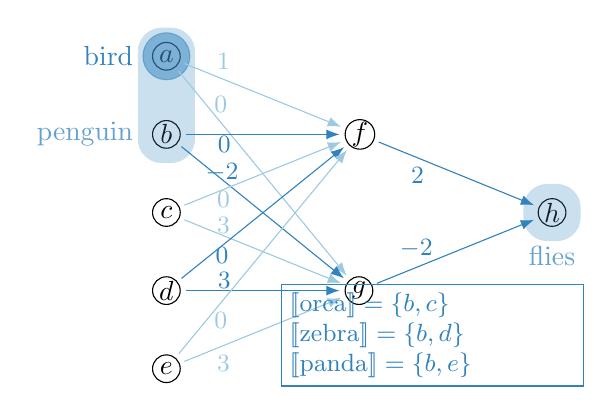
\begin{tikzpicture}[loose/.style={inner sep=.7em},edge/.style = {->,-Latex},
oval/.style={ellipse,draw}]

% nodes
\node[circle,minimum size=10pt,inner sep=0pt,outer sep=2pt,fill=white,draw](a){$a$};
\node[below=0.5 of a,circle,minimum size=10pt,inner sep=0pt,outer sep=2pt,fill=white,draw](b){$b$};
\node[below=0.5 of b,circle,minimum size=10pt,inner sep=0pt,outer sep=2pt,fill=white,draw](c){$c$};
\node[below=0.5 of c,circle,minimum size=10pt,inner sep=0pt,outer sep=2pt,fill=white,draw](d){$d$};
\node[below=0.5 of d,circle,minimum size=10pt,inner sep=0pt,outer sep=2pt,fill=white,draw](e){$e$};

\node[right=2.2 of $(a)!0.5!(c)$,circle,minimum size=10pt,inner sep=0pt,outer sep=2pt,fill=white,draw](f){$f$};
\node[right=2.2 of $(c)!0.5!(e)$,circle,minimum size=10pt,inner sep=0pt,outer sep=2pt,fill=white,draw](g){$g$};

\node[right=2.2 of $(f)!0.5!(g)$,circle,minimum size=10pt,inner sep=0pt,outer sep=2pt,fill=white,draw](h){$h$};

% Hidden nodes
\node (bpivot) [left=0.3 of b] {\phantom{p}};
\node (dpivot) [left=0.3 of d] {\phantom{p}};
\node (bpivot2) [right=0.3 of b] {\phantom{p}};
\node (epivot) [right=0.3 of e] {\phantom{p}};

% sets
\node[fill=myblue2,color=myblue2, opacity=0.5,oval,fit=(a),inner sep=-1pt]{};
\node[fill=myblue2, opacity=0.25,rectangle,rounded corners=2ex,fit=(a) (b)]{};
\node[fill=myblue2, opacity=0.25,rectangle,rounded corners=2ex,fit=(h)]{};


% set labels
\node [color=myblue2,opacity=1,left=0.3 of $(a)$]{bird};
\node [color=myblue2,opacity=0.75,left=0.3 of $(b)$]{penguin};
\node [color=myblue2,opacity=0.75,below=0.3 of $(h)$]{flies};

\draw[edge, color=myblue1] (a) -- (f) node [near start, above] {\small{\textbf{$1$}}};
\draw[edge, color=myblue1] (a) -- (g) node [near start, above] {\small{\textbf{$0$}}};
\draw[edge, color=myblue2] (b) -- (f) node [below=-0.1, near start] {\small{\textbf{$0$}}};
\draw[edge, color=myblue2] (b) -- (g) node [near start, above=-0.15] {\small{\textbf{$-2$}}};
\draw[edge, color=myblue1] (c) -- (f) node [near start, below=-0.1] {\small{\textbf{$0$}}};
\draw[edge, color=myblue1] (c) -- (g) node [near start, above=-0.1] {\small{\textbf{$3$}}};
\draw[edge, color=myblue2] (d) -- (f) node [near start, below=-0.1] {\small{\textbf{$0$}}};
\draw[edge, color=myblue2] (d) -- (g) node [near start, above=-0.1] {\small{\textbf{$3$}}};
\draw[edge, color=myblue1] (e) -- (f) node [near start, below] {\small{\textbf{$0$}}};
\draw[edge, color=myblue1] (e) -- (g) node [near start, below] {\small{\textbf{$3$}}};
\draw[edge, color=myblue2] (f) -- (h) node [near start, below] {\small{\textbf{$2$}}};
\draw[edge, color=myblue2] (g) -- (h) node [near start, above] {\small{\textbf{$-2$}}};

% KEY
\node[draw, color=myblue2, text width=0.30\linewidth,inner sep=1mm,align=left,
      above left] at (current bounding box.south east)
    {\small $\semantics{\textup{orca}} = \set{b, c}$\\
    $\semantics{\textup{zebra}} = \set{b, d}$\\
    $\semantics{\textup{panda}} = \set{b, e}$\\};

\end{tikzpicture}
}
\caption{A BFNN $\Net$, equipped with the ReLU activation function, $T = 1$, and $\eta = 1$.  After observing the dataset $\langle \textrm{orca}, \textrm{zebra}, \textrm{panda} \rangle$, $\Net$ learns that penguins do not fly, while preserving the fact that birds typically fly.}
\label{fig:full-example}
\end{figure}

We now demonstrate our neuro-symbolic interface by way of an example neural network in a machine learning context.  The task: Given an image of an animal, classify it as flying or non-flying.  Suppose we have the partially pre-trained BFNN $\Net$ in  Figure~\ref{fig:full-example}.  

For simplification's sake, let's suppose that our animal images can be reduced to $5$-dimensional vectors in order to be fed into the input layer of $\Net$.  Say:
\[
\begin{array}{llcll}
\textrm{penguin} & \langle 1 1 0 0 0 \rangle & \quad & 
\textrm{orca} & \langle 0 1 1 0 0 \rangle \\
\textrm{zebra} & \langle 0 1 0 1 0 \rangle & \quad & 
\textrm{panda} & \langle 0 1 0 0 1 \rangle \\
\end{array}
\]
In addition, suppose an image activates the first node if and only if it depicts a bird.

We can identify each animal with the set of nodes it activates in the input layer.  This gives us the sets shown in Figure~\ref{fig:full-example}.  We can also identify the class of things that fly with the output node, i.e. $\semantics{\textup{flies}} = \set{h}$.  In principle we can identify propositions with sets containing hidden nodes as well, although in practice the meaning of hidden nodes is often unclear.

With this interpretation in mind, we see that $\Net \models \textrm{bird} \Rightarrow \textrm{flies}$, but also $\Net \models \textrm{penguin} \Rightarrow \textrm{flies}$ (which is incorrect).  Our hope is that $\Net$ corrects this mistake via Hebbian learning.

Say we expose $\Net$ to non-flying animals that share the black-and-white color of penguins, e.g. we train $\Net$ on the dataset $\langle \textrm{orca}, \textrm{zebra}, \textrm{panda} \rangle$.  The propagations of each instance will increase $W_{bg}$.  Once we have given $\Net$ the entire dataset ($W_{bg} = 1$), $\Prop(\semantics{\textup{penguin}})$ will contain $g$, which will cancel the signal given by ${f \to h}$.  Our logic successfully models this behavior:
\[
\begin{array}{l}
\Net \models [\textrm{orca}^+] [\textrm{zebra}^+] [\textrm{panda}^+] (\textrm{bird} \Rightarrow \textrm{flies}) \textrm{, yet}\\
\Net \not \models [\textrm{orca}^+] [\textrm{zebra}^+] [\textrm{panda}^+] (\textrm{penguin} \Rightarrow \textrm{flies})
\end{array}
\]
i.e. $\Net$ learns that penguins do not fly while preserving the fact that birds typically fly. 

As it happens, if we modify $\Net$ such that $W_{bg} = 0$ then this serves as a counterexample to monotonicity in $S$ (see the discussion following Theorem~\ref{thm:inc-props}).  In particular, we have $\Net \models \Typ(\textrm{penguin}) \to \textrm{flies}$, yet $\Net \not \models [\textrm{orca}^+] \Typ(\textrm{penguin}) \to [\textrm{orca}^+] \textrm{flies}$. 

%%%%%%%%%%%%%%%%%%%%%%%%%%%%%%%%%%%%%%%%%%%%
\section{Conclusion and Future Work}

In this paper, we gave sound axioms and rules characterizing the logic of Hebbian learning.  This logic interfaces the neuro-symbolic divide by characterizing conditionals $\Rightarrow$ and modalities $\Typ$, $[\varphi^+]$ in terms of the propagation and Hebbian update of signals in a neural network.  The upshot of all this is that this logic describes a neuro-symbolic agent that learns associatively and also reasons about what it has learned.

We leave open the question of whether the axioms and rules we list are complete.  But we take this opportunity to stress the importance of having strong completeness for logics of this kind.  Strong completeness for a \emph{static} neural semantics provides a bridge across which we can extract a set of rules $\Gamma$ from an interpreted network, and also build an interpreted neural network implementing $\Gamma$.  But once the neural network updates, we lose the interpretations of neurons that allow for these translations.  If we had strong completeness for the \emph{dynamic} logic, we could fully track the interpretations while the net learns and preserve this neuro-symbolic correspondence.

% SAVE CONSIDERATION FOR JOURNAL VERSION
% In order to obtain a complete set of axioms, we might look at logics of preference upgrade for inspiration.  In Related Work we mentioned that, as with our $[\varphi^+]$, the modalities $[{\Uparrow} \varphi]$ and $[{\uparrow} \varphi]$ of preference upgrade logic are characterized by their interaction with conditionals $\Rightarrow$.  So we should consider whether $[\varphi^+]$ interacts with conditionals in the same way.  Unfortunately, the reduction axiom for lexicographic upgrade $[{\Uparrow} \varphi]$ (expressed in our language and written to avoid nested implications)
% \begin{multline*}
% \proves [\varphi^+] (\psi \Rightarrow \rho) \quad \textrm{iff} \\
% \quad \proves (\neg (\varphi \land [\varphi^+] \psi \leftrightarrow \top)
% \land (\varphi \land [\varphi^+] \psi \Rightarrow [\varphi^+] \rho))\\
% \orr ((\varphi \land [\varphi^+] \psi \leftrightarrow \top) \land ([\varphi^+] \psi \Rightarrow [\varphi^+] \rho))
% \end{multline*}
% is not sound in our logic.  The same is true of  the reduction for elite change $[{\uparrow} \varphi]$.  So we should consider different strategies for completeness of our logic.

Beyond the logic of Hebbian learning, we believe that this framework will be a fruitful way to explore the neuro-symbolic interface for a variety of neural networks and learning policies.  Exciting future directions include:
\begin{enumerate}[itemsep=-1pt, topsep=2pt]
    \item Mapping more expressive syntax to neural activity
    \item Generalizing to a broader class of neural networks
    \item Generalizing to a broader class of activation functions
    \item Characterizing other learning policies in logical terms
\end{enumerate}
The holy grail of this line of work is to completely axiomatize the (1) first-order logic of (2) nonbinary (fuzzy-valued) neural networks with (3) more varied (e.g. ReLU and GELU) activation functions that (4) learn via backpropagation.

\section{Acknowledgements} We thank the anonymous reviewers for their careful reviews and helpful comments.  Additionally, C.~Kisby was supported in part by the US Department of Defense [Contract No. W52P1J2093009].

\bibliographystyle{flairs}
\bibliography{kisby-blanco-moss}

\definecolor{iucolor1}{RGB}{105,3,4}
\definecolor{iucolor2}{RGB}{168,29,54}
\definecolor{iucolor3}{RGB}{64,64,65}


% % BASE FRAME
% \centering{
% \begin{tikzpicture}[loose/.style={inner sep=.7em},edge/.style = {->,-Latex},
% oval/.style={ellipse,draw}]
% \node[circle,minimum size=10pt,inner sep=0pt,outer sep=2pt,fill=white,draw](a){};
% \node[below=0.5 of a,circle,minimum size=10pt,inner sep=0pt,outer sep=2pt,fill=white,draw](b){};
% \node[below=0.5 of b,circle,minimum size=10pt,inner sep=0pt,outer sep=2pt,fill=white,draw](c){};
% \node[below=0.5 of c,circle,minimum size=10pt,inner sep=0pt,outer sep=2pt,fill=white,draw](d){};
% \node[below=0.5 of d,circle,minimum size=10pt,inner sep=0pt,outer sep=2pt,fill=white,draw](e){};
% \node[right=2.2 of $(a)!0.5!(c)$,circle,minimum size=10pt,inner sep=0pt,outer sep=2pt,fill=white,draw](f){};
% \node[right=2.2 of $(b)!0.5!(d)$,circle,minimum size=10pt,inner sep=0pt,outer sep=2pt,fill=white,draw](g){};
% \node[right=2.2 of $(c)!0.5!(e)$,circle,minimum size=10pt,inner sep=0pt,outer sep=2pt,fill=white,draw](h){};
% \node[right=2.2 of $(f)!0.5!(h)$,circle,minimum size=10pt,inner sep=0pt,outer sep=2pt,fill=white,draw](i){};
% \node (bpivot) [left=0.3 of b] {\phantom{p}};
% \node (dpivot) [left=0.3 of d] {\phantom{p}};
% \node (bpivot2) [right=0.3 of b] {\phantom{p}};
% \node (epivot) [right=0.3 of e] {\phantom{p}};

% % Prop update
% \node[fill=iucolor2, opacity=0.45,rectangle,rounded corners=2ex,fit=(a) (b), inner sep=1pt]{};
% \node[fill=iucolor1, opacity=0.45,rectangle,rounded corners=2ex,fit=(a) (b) (c) (d), inner sep=2pt]{};

% \node [color=black,opacity=0.75,below=0.3 of $(i)$]{flies};
% \draw[edge, color=black] (a) -- (f) node [near start, above] {};
% \draw[edge, color=black] (a) -- (g) node [near start, above] {};
% \draw[edge, color=black] (a) -- (h) node [near start, above] {};
% \draw[edge, color=black] (b) -- (f) node [below=-0.1, near start] {};
% \draw[edge, color=black] (b) -- (g) node [near start, above=-0.15] {};
% \draw[edge, color=black] (b) -- (h) node [near start, above=-0.15] {};
% \draw[edge, color=black] (c) -- (f) node [near start, below=-0.1] {};
% \draw[edge, color=black] (c) -- (g) node [near start, above=-0.1] {};
% \draw[edge, color=black] (c) -- (h) node [near start, above=-0.1] {};
% \draw[edge, color=black] (d) -- (f) node [near start, below=-0.1] {};
% \draw[edge, color=black] (d) -- (g) node [near start, above=-0.1] {};
% \draw[edge, color=black] (d) -- (h) node [near start, above=-0.1] {};
% \draw[edge, color=black] (e) -- (f) node [near start, below] {};
% \draw[edge, color=black] (e) -- (g) node [near start, below] {};
% \draw[edge, color=black] (e) -- (h) node [near start, below] {};
% \draw[edge, color=black] (f) -- (i) node [near start, below] {};
% \draw[edge, color=black] (g) -- (i) node [near start, above] {};
% \draw[edge, color=black] (h) -- (i) node [near start, above] {};
% \end{tikzpicture}
% }

% % Conditional example
% \centering{
% \begin{tikzpicture}[loose/.style={inner sep=.7em},edge/.style = {->,-Latex},
% oval/.style={ellipse,draw}]
% \node[circle,minimum size=10pt,inner sep=0pt,outer sep=2pt,fill=white,draw](a){};
% \node[below=0.5 of a,circle,minimum size=10pt,inner sep=0pt,outer sep=2pt,fill=white,draw](b){};
% \node[below=0.5 of b,circle,minimum size=10pt,inner sep=0pt,outer sep=2pt,fill=white,draw](c){};
% \node[below=0.5 of c,circle,minimum size=10pt,inner sep=0pt,outer sep=2pt,fill=white,draw](d){};
% \node[below=0.5 of d,circle,minimum size=10pt,inner sep=0pt,outer sep=2pt,fill=white,draw](e){};
% \node[right=2.2 of $(a)!0.5!(c)$,circle,minimum size=10pt,inner sep=0pt,outer sep=2pt,fill=white,draw](f){};
% \node[right=2.2 of $(b)!0.5!(d)$,circle,minimum size=10pt,inner sep=0pt,outer sep=2pt,fill=white,draw](g){};
% \node[right=2.2 of $(c)!0.5!(e)$,circle,minimum size=10pt,inner sep=0pt,outer sep=2pt,fill=white,draw](h){};
% \node[right=2.2 of $(f)!0.5!(h)$,circle,minimum size=10pt,inner sep=0pt,outer sep=2pt,fill=white,draw](i){};
% \node (bpivot) [left=0.3 of b] {\phantom{p}};
% \node (dpivot) [left=0.3 of d] {\phantom{p}};
% \node (bpivot2) [right=0.3 of b] {\phantom{p}};
% \node (epivot) [right=0.3 of e] {\phantom{p}};

% % Prop update
% % 1
% \node[fill=iucolor2, opacity=0.7,rectangle,rounded corners=2ex,fit=(a) (b), inner sep=2pt]{};
% % 2
% \node[fill=iucolor2, opacity=0.7,rectangle,rounded corners=2ex,fit=(f), inner sep=2pt]{};
% \node[fill=iucolor2, opacity=0.7,rectangle,rounded corners=2ex,fit=(h), inner sep=2pt]{};
% % 3
% \node[fill=iucolor2, opacity=0.7,rectangle,rounded corners=2ex,fit=(i), inner sep=2pt]{};

% \node [color=black,opacity=0.75,below=0.3 of $(i)$]{flies};
% \draw[edge, color=black] (a) -- (f) node [near start, above] {};
% \draw[edge, color=black] (a) -- (g) node [near start, above] {};
% \draw[edge, color=black] (a) -- (h) node [near start, above] {};
% \draw[edge, color=black] (b) -- (f) node [below=-0.1, near start] {};
% \draw[edge, color=black] (b) -- (g) node [near start, above=-0.15] {};
% \draw[edge, color=black] (b) -- (h) node [near start, above=-0.15] {};
% \draw[edge, color=black] (c) -- (f) node [near start, below=-0.1] {};
% \draw[edge, color=black] (c) -- (g) node [near start, above=-0.1] {};
% \draw[edge, color=black] (c) -- (h) node [near start, above=-0.1] {};
% \draw[edge, color=black] (d) -- (f) node [near start, below=-0.1] {};
% \draw[edge, color=black] (d) -- (g) node [near start, above=-0.1] {};
% \draw[edge, color=black] (d) -- (h) node [near start, above=-0.1] {};
% \draw[edge, color=black] (e) -- (f) node [near start, below] {};
% \draw[edge, color=black] (e) -- (g) node [near start, below] {};
% \draw[edge, color=black] (e) -- (h) node [near start, below] {};
% \draw[edge, color=black] (f) -- (i) node [near start, below] {};
% \draw[edge, color=black] (g) -- (i) node [near start, above] {};
% \draw[edge, color=black] (h) -- (i) node [near start, above] {};
% \end{tikzpicture}
% }



% % NOT ANIMATED -- just show two different nets with different propagations for penguin
% \centering{
% \begin{tikzpicture}[loose/.style={inner sep=.7em},edge/.style = {->,-Latex},
% oval/.style={ellipse,draw}]
% \node[circle,minimum size=10pt,inner sep=0pt,outer sep=2pt,fill=white,draw](a){};
% \node[below=0.5 of a,circle,minimum size=10pt,inner sep=0pt,outer sep=2pt,fill=white,draw](b){};
% \node[below=0.5 of b,circle,minimum size=10pt,inner sep=0pt,outer sep=2pt,fill=white,draw](c){};
% \node[below=0.5 of c,circle,minimum size=10pt,inner sep=0pt,outer sep=2pt,fill=white,draw](d){};
% \node[below=0.5 of d,circle,minimum size=10pt,inner sep=0pt,outer sep=2pt,fill=white,draw](e){};
% \node[right=2.2 of $(a)!0.5!(c)$,circle,minimum size=10pt,inner sep=0pt,outer sep=2pt,fill=white,draw](f){};
% \node[right=2.2 of $(b)!0.5!(d)$,circle,minimum size=10pt,inner sep=0pt,outer sep=2pt,fill=white,draw](g){};
% \node[right=2.2 of $(c)!0.5!(e)$,circle,minimum size=10pt,inner sep=0pt,outer sep=2pt,fill=white,draw](h){};
% \node[right=2.2 of $(f)!0.5!(h)$,circle,minimum size=10pt,inner sep=0pt,outer sep=2pt,fill=white,draw](i){};
% \node (bpivot) [left=0.3 of b] {\phantom{p}};
% \node (dpivot) [left=0.3 of d] {\phantom{p}};
% \node (bpivot2) [right=0.3 of b] {\phantom{p}};
% \node (epivot) [right=0.3 of e] {\phantom{p}};

% % Prop update
% \node[fill=iucolor2, opacity=0.45,rectangle,rounded corners=2ex,fit=(a) (b), inner sep=1pt]{};
% \node[fill=iucolor1, opacity=0.45,rectangle,rounded corners=2ex,fit=(a) (b) (c) (d), inner sep=2pt]{};
% \node[fill=iucolor1, opacity=0.45,rectangle,rounded corners=2ex,fit=(f), inner sep=2pt]{};
% \node[fill=iucolor1, opacity=0.45,rectangle,rounded corners=2ex,fit=(g), inner sep=2pt]{};
% \node[fill=iucolor1, opacity=0.45,rectangle,rounded corners=2ex,fit=(h), inner sep=2pt]{};

% \node [color=black,opacity=0.75,below=0.3 of $(i)$]{flies};
% \draw[edge, color=black] (a) -- (f) node [near start, above] {};
% \draw[edge, color=black] (a) -- (g) node [near start, above] {};
% \draw[edge, color=black] (a) -- (h) node [near start, above] {};
% \draw[edge, color=black] (b) -- (f) node [below=-0.1, near start] {};
% \draw[edge, color=black] (b) -- (g) node [near start, above=-0.15] {};
% \draw[edge, color=black] (b) -- (h) node [near start, above=-0.15] {};
% \draw[edge, color=black] (c) -- (f) node [near start, below=-0.1] {};
% \draw[edge, color=black] (c) -- (g) node [near start, above=-0.1] {};
% \draw[edge, color=black] (c) -- (h) node [near start, above=-0.1] {};
% \draw[edge, color=black] (d) -- (f) node [near start, below=-0.1] {};
% \draw[edge, color=red, line width=1pt] (d) -- (g) node [near start, above=-0.1] {};
% \draw[edge, color=black] (d) -- (h) node [near start, above=-0.1] {};
% \draw[edge, color=black] (e) -- (f) node [near start, below] {};
% \draw[edge, color=black] (e) -- (g) node [near start, below] {};
% \draw[edge, color=black] (e) -- (h) node [near start, below] {};
% \draw[edge, color=black] (f) -- (i) node [near start, below] {};
% \draw[edge, color=red, line width=1pt] (g) -- (i) node [near start, above] {\small $-100$};
% \draw[edge, color=black] (h) -- (i) node [near start, above] {};
% \end{tikzpicture}
% }

% % NOT ANIMATED -- just show two different nets with different propagations for penguin
% \centering{
% \begin{tikzpicture}[loose/.style={inner sep=.7em},edge/.style = {->,-Latex},
% oval/.style={ellipse,draw}]
% \node[circle,minimum size=10pt,inner sep=0pt,outer sep=2pt,fill=white,draw](a){};
% \node[below=0.5 of a,circle,minimum size=10pt,inner sep=0pt,outer sep=2pt,fill=white,draw](b){};
% \node[below=0.5 of b,circle,minimum size=10pt,inner sep=0pt,outer sep=2pt,fill=white,draw](c){};
% \node[below=0.5 of c,circle,minimum size=10pt,inner sep=0pt,outer sep=2pt,fill=white,draw](d){};
% \node[below=0.5 of d,circle,minimum size=10pt,inner sep=0pt,outer sep=2pt,fill=white,draw](e){};
% \node[right=2.2 of $(a)!0.5!(c)$,circle,minimum size=10pt,inner sep=0pt,outer sep=2pt,fill=white,draw](f){};
% \node[right=2.2 of $(b)!0.5!(d)$,circle,minimum size=10pt,inner sep=0pt,outer sep=2pt,fill=white,draw](g){};
% \node[right=2.2 of $(c)!0.5!(e)$,circle,minimum size=10pt,inner sep=0pt,outer sep=2pt,fill=white,draw](h){};
% \node[right=2.2 of $(f)!0.5!(h)$,circle,minimum size=10pt,inner sep=0pt,outer sep=2pt,fill=white,draw](i){};
% \node (bpivot) [left=0.3 of b] {\phantom{p}};
% \node (dpivot) [left=0.3 of d] {\phantom{p}};
% \node (bpivot2) [right=0.3 of b] {\phantom{p}};
% \node (epivot) [right=0.3 of e] {\phantom{p}};

% % Prop update
% \node[fill=iucolor2, opacity=0.45,rectangle,rounded corners=2ex,fit=(a) (b), inner sep=1pt]{};
% \node[fill=iucolor1, opacity=0.45,rectangle,rounded corners=2ex,fit=(a) (b) (c) (d), inner sep=2pt]{};
% \node[fill=iucolor1, opacity=0.45,rectangle,rounded corners=2ex,fit=(f), inner sep=2pt]{};
% \node[fill=iucolor1, opacity=0.45,rectangle,rounded corners=2ex,fit=(h), inner sep=2pt]{};
% \node[fill=iucolor1, opacity=0.45,rectangle,rounded corners=2ex,fit=(i), inner sep=2pt]{};

% \node [color=black,opacity=0.75,below=0.3 of $(i)$]{flies};
% \draw[edge, color=black] (a) -- (f) node [near start, above] {};
% \draw[edge, color=black] (a) -- (g) node [near start, above] {};
% \draw[edge, color=black] (a) -- (h) node [near start, above] {};
% \draw[edge, color=black] (b) -- (f) node [below=-0.1, near start] {};
% \draw[edge, color=black] (b) -- (g) node [near start, above=-0.15] {};
% \draw[edge, color=black] (b) -- (h) node [near start, above=-0.15] {};
% \draw[edge, color=black] (c) -- (f) node [near start, below=-0.1] {};
% \draw[edge, color=black] (c) -- (g) node [near start, above=-0.1] {};
% \draw[edge, color=black] (c) -- (h) node [near start, above=-0.1] {};
% \draw[edge, color=black] (d) -- (f) node [near start, below=-0.1] {};
% \draw[edge, color=black] (d) -- (g) node [near start, above=-0.1] {};
% \draw[edge, color=black] (d) -- (h) node [near start, above=-0.1] {};
% \draw[edge, color=black] (e) -- (f) node [near start, below] {};
% \draw[edge, color=black] (e) -- (g) node [near start, below] {};
% \draw[edge, color=black] (e) -- (h) node [near start, below] {};
% \draw[edge, color=black] (f) -- (i) node [near start, below] {};
% \draw[edge, color=black] (g) -- (i) node [near start, above] {};
% \draw[edge, color=black] (h) -- (i) node [near start, above] {};
% \end{tikzpicture}
% }

% \[
% \boxed{
% \begin{array}{l}
% \mbox{penguin} \to \mbox{bird}\\
% \mbox{bird} \Rightarrow \mbox{flies}\\
% \neg (\mbox{penguin} \Rightarrow \mbox{flies})
% \end{array}
% }
% \]


% \[
% \boxed{
% \mbox{bird} \Rightarrow \mbox{flies} \quad \mbox{iff} \quad \Prop(\semantics{\textnormal{bird}}) \supseteq \semantics{\textnormal{flies}}
% }
% \]

% \[
% \boxed{
% \varphi \Rightarrow \psi \quad \mbox{iff} \quad \Prop(\semantics{\varphi}) \supseteq \semantics{\psi}
% }
% \]

% \[
% \Delta W_{ij} = \eta x_i x_j
% \]

% \[
% \forall x P(x), \exists x P(x)
% \]


% % ORCA EXAMPLE
% \centering{
% \begin{tikzpicture}[loose/.style={inner sep=.7em},edge/.style = {->,-Latex},
% oval/.style={ellipse,draw}]
% \node[circle,minimum size=10pt,inner sep=0pt,outer sep=2pt,fill=white,draw](a){};
% \node[below=0.5 of a,circle,minimum size=10pt,inner sep=0pt,outer sep=2pt,fill=white,draw](b){};
% \node[below=0.5 of b,circle,minimum size=10pt,inner sep=0pt,outer sep=2pt,fill=white,draw](c){};
% \node[below=0.5 of c,circle,minimum size=10pt,inner sep=0pt,outer sep=2pt,fill=white,draw](d){};
% \node[below=0.5 of d,circle,minimum size=10pt,inner sep=0pt,outer sep=2pt,fill=white,draw](e){};
% \node[right=2.2 of $(a)!0.5!(c)$,circle,minimum size=10pt,inner sep=0pt,outer sep=2pt,fill=white,draw](f){};
% \node[right=2.2 of $(b)!0.5!(d)$,circle,minimum size=10pt,inner sep=0pt,outer sep=2pt,fill=white,draw](g){};
% \node[right=2.2 of $(c)!0.5!(e)$,circle,minimum size=10pt,inner sep=0pt,outer sep=2pt,fill=white,draw](h){};
% \node[right=2.2 of $(f)!0.5!(h)$,circle,minimum size=10pt,inner sep=0pt,outer sep=2pt,fill=white,draw](i){};
% \node (bpivot) [left=0.3 of b] {\phantom{p}};
% \node (dpivot) [left=0.3 of d] {\phantom{p}};
% \node (bpivot2) [right=0.3 of b] {\phantom{p}};
% \node (epivot) [right=0.3 of e] {\phantom{p}};

% % Prop update
% \node[fill=iucolor3, opacity=0.7,rectangle,rounded corners=2ex,fit=(d) (e), inner sep=2pt]{};
% % \node[fill=iucolor3, opacity=0.7,rectangle,rounded corners=2ex,fit=(f), inner sep=2pt]{};
% % \node[fill=iucolor3, opacity=0.7,rectangle,rounded corners=2ex,fit=(g), inner sep=2pt]{};
% % \node[fill=iucolor3, opacity=0.7,rectangle,rounded corners=2ex,fit=(h), inner sep=2pt]{};

% \node [color=black,opacity=0.75,below=0.3 of $(i)$]{flies};
% \draw[edge, color=black] (a) -- (f) node [near start, above] {};
% \draw[edge, color=black] (a) -- (g) node [near start, above] {};
% \draw[edge, color=black] (a) -- (h) node [near start, above] {};
% \draw[edge, color=black] (b) -- (f) node [below=-0.1, near start] {};
% \draw[edge, color=black] (b) -- (g) node [near start, above=-0.15] {};
% \draw[edge, color=black] (b) -- (h) node [near start, above=-0.15] {};
% \draw[edge, color=black] (c) -- (f) node [near start, below=-0.1] {};
% \draw[edge, color=black] (c) -- (g) node [near start, above=-0.1] {};
% \draw[edge, color=black] (c) -- (h) node [near start, above=-0.1] {};

% \draw[edge, color=black] (d) -- (f) node [near start, below=-0.1] {};
% \draw[edge, color=black] (d) -- (g) node [near start, above=-0.1] {};
% \draw[edge, color=black] (d) -- (h) node [near start, above=-0.1] {};

% % \draw[edge, color=red, line width=1pt] (d) -- (f) node [near start, below=-0.1] {};
% % \draw[edge, color=red, line width=1pt] (d) -- (g) node [near start, above=-0.1] {};
% % \draw[edge, color=red, line width=1pt] (d) -- (h) node [near start, above=-0.1] {};


% \draw[edge, color=black] (e) -- (f) node [near start, below] {};
% \draw[edge, color=black] (e) -- (g) node [near start, below] {};
% \draw[edge, color=black] (e) -- (h) node [near start, below] {};

% % \draw[edge, color=red, line width=1pt] (e) -- (f) node [near start, below] {};
% % \draw[edge, color=red, line width=1pt] (e) -- (g) node [near start, below] {};
% % \draw[edge, color=red, line width=1pt] (e) -- (h) node [near start, below] {};

% \draw[edge, color=black] (f) -- (i) node [near start, below] {};
% \draw[edge, color=black] (g) -- (i) node [near start, above] {\small $-100$};
% \draw[edge, color=black] (h) -- (i) node [near start, above] {};
% \end{tikzpicture}
% }




% \centering{
% \begin{tikzpicture}[loose/.style={inner sep=.7em},edge/.style = {->,-Latex},
% oval/.style={ellipse,draw}]
% \node[circle,minimum size=10pt,inner sep=0pt,outer sep=2pt,fill=white,draw](a){};
% \node[below=0.5 of a,circle,minimum size=10pt,inner sep=0pt,outer sep=2pt,fill=white,draw](b){};
% \node[below=0.5 of b,circle,minimum size=10pt,inner sep=0pt,outer sep=2pt,fill=white,draw](c){};
% \node[below=0.5 of c,circle,minimum size=10pt,inner sep=0pt,outer sep=2pt,fill=white,draw](d){};
% \node[below=0.5 of d,circle,minimum size=10pt,inner sep=0pt,outer sep=2pt,fill=white,draw](e){};
% \node[right=2.2 of $(a)!0.5!(c)$,circle,minimum size=10pt,inner sep=0pt,outer sep=2pt,fill=white,draw](f){};
% \node[right=2.2 of $(b)!0.5!(d)$,circle,minimum size=10pt,inner sep=0pt,outer sep=2pt,fill=white,draw](g){};
% \node[right=2.2 of $(c)!0.5!(e)$,circle,minimum size=10pt,inner sep=0pt,outer sep=2pt,fill=white,draw](h){};
% \node[right=2.2 of $(f)!0.5!(h)$,circle,minimum size=10pt,inner sep=0pt,outer sep=2pt,fill=white,draw](i){};
% \node (bpivot) [left=0.3 of b] {\phantom{p}};
% \node (dpivot) [left=0.3 of d] {\phantom{p}};
% \node (bpivot2) [right=0.3 of b] {\phantom{p}};
% \node (epivot) [right=0.3 of e] {\phantom{p}};

% \draw[edge, color=black] (a) -- (f) node [near start, above] {};
% \draw[edge, color=black] (a) -- (g) node [near start, above] {};
% \draw[edge, color=black] (a) -- (h) node [near start, above] {};
% \draw[edge, color=black] (b) -- (f) node [below=-0.1, near start] {};
% \draw[edge, color=black] (b) -- (g) node [near start, above=-0.15] {};
% \draw[edge, color=black] (b) -- (h) node [near start, above=-0.15] {};
% \draw[edge, color=black] (c) -- (f) node [near start, below=-0.1] {};
% \draw[edge, color=black] (c) -- (g) node [near start, above=-0.1] {};
% \draw[edge, color=black] (c) -- (h) node [near start, above=-0.1] {};

% \draw[edge, color=black] (d) -- (f) node [near start, below=-0.1] {};
% \draw[edge, color=black] (d) -- (g) node [near start, above=-0.1] {};
% \draw[edge, color=black] (d) -- (h) node [near start, above=-0.1] {};


% \draw[edge, color=black] (e) -- (f) node [near start, below] {};
% \draw[edge, color=black] (e) -- (g) node [near start, below] {};
% \draw[edge, color=black] (e) -- (h) node [near start, below] {};

% % \draw[edge, color=red, line width=1pt] (e) -- (f) node [near start, below] {};
% % \draw[edge, color=red, line width=1pt] (e) -- (g) node [near start, below] {};
% % \draw[edge, color=red, line width=1pt] (e) -- (h) node [near start, below] {};

% \draw[edge, color=black] (f) -- (i) node [near start, below] {};
% \draw[edge, color=black] (g) -- (i) node [near start, above] {};
% \draw[edge, color=black] (h) -- (i) node [near start, above] {};
% \end{tikzpicture}
% }



% \[
% \begin{array}{l}
% \Prop : \Set \to \Set\\
% \Prop(S) \mbox{ means } \textit{forward-propagate } S \mbox{ in the net.}\\
% \\
% \Inc : \AllNets \times \Set \to \AllNets\\
% \Inc(\Net, S) \mbox{ means } \textit{increase the weights } \mbox{of edges within }\\
% \quad \quad \quad \quad \quad \quad \quad \quad \Prop(S) \mbox{ by } \Delta W_{ij} = \eta x_i x_j
% \end{array}
% \]


% \begin{figure}
% \centering{
% \begin{tikzpicture}[loose/.style={inner sep=.7em},edge/.style = {->,-Latex},
% oval/.style={ellipse,draw}]

% % nodes
% \node[circle,minimum size=10pt,inner sep=0pt,outer sep=2pt,fill=white,draw](a){$a$};
% \node[below=0.5 of a,circle,minimum size=10pt,inner sep=0pt,outer sep=2pt,fill=white,draw](b){$b$};
% \node[below=0.5 of b,circle,minimum size=10pt,inner sep=0pt,outer sep=2pt,fill=white,draw](c){$c$};
% \node[below=0.5 of c,circle,minimum size=10pt,inner sep=0pt,outer sep=2pt,fill=white,draw](d){$d$};
% \node[below=0.5 of d,circle,minimum size=10pt,inner sep=0pt,outer sep=2pt,fill=white,draw](e){$e$};

% \node[right=2.2 of $(a)!0.5!(c)$,circle,minimum size=10pt,inner sep=0pt,outer sep=2pt,fill=white,draw](f){$f$};
% \node[right=2.2 of $(c)!0.5!(e)$,circle,minimum size=10pt,inner sep=0pt,outer sep=2pt,fill=white,draw](g){$g$};

% \node[right=2.2 of $(f)!0.5!(g)$,circle,minimum size=10pt,inner sep=0pt,outer sep=2pt,fill=white,draw](h){$h$};

% % Hidden nodes
% \node (bpivot) [left=0.3 of b] {\phantom{p}};
% \node (dpivot) [left=0.3 of d] {\phantom{p}};
% \node (bpivot2) [right=0.3 of b] {\phantom{p}};
% \node (epivot) [right=0.3 of e] {\phantom{p}};

% % sets
% \node[fill=iucolor2,color=iucolor2, opacity=0.5,oval,fit=(a),inner sep=-1pt]{};
% \node[fill=iucolor2, opacity=0.25,rectangle,rounded corners=2ex,fit=(a) (b)]{};
% \node[fill=iucolor2, opacity=0.25,rectangle,rounded corners=2ex,fit=(h)]{};


% % set labels
% \node [color=iucolor2,opacity=1,left=0.3 of $(a)$]{bird};
% \node [color=iucolor2,opacity=0.75,left=0.3 of $(b)$]{penguin};
% \node [color=iucolor2,opacity=0.75,below=0.3 of $(h)$]{flies};

% \draw[edge, color=iucolor1] (a) -- (f) node [near start, above] {\small{\textbf{$1$}}};
% \draw[edge, color=iucolor1] (a) -- (g) node [near start, above] {\small{\textbf{$0$}}};
% \draw[edge, color=iucolor2] (b) -- (f) node [below=-0.1, near start] {\small{\textbf{$0$}}};
% \draw[edge, color=iucolor2] (b) -- (g) node [near start, above=-0.15] {\small{\textbf{$-2$}}};
% \draw[edge, color=iucolor1] (c) -- (f) node [near start, below=-0.1] {\small{\textbf{$0$}}};
% \draw[edge, color=iucolor1] (c) -- (g) node [near start, above=-0.1] {\small{\textbf{$3$}}};
% \draw[edge, color=iucolor2] (d) -- (f) node [near start, below=-0.1] {\small{\textbf{$0$}}};
% \draw[edge, color=iucolor2] (d) -- (g) node [near start, above=-0.1] {\small{\textbf{$3$}}};
% \draw[edge, color=iucolor1] (e) -- (f) node [near start, below] {\small{\textbf{$0$}}};
% \draw[edge, color=iucolor1] (e) -- (g) node [near start, below] {\small{\textbf{$3$}}};
% \draw[edge, color=iucolor2] (f) -- (h) node [near start, below] {\small{\textbf{$2$}}};
% \draw[edge, color=iucolor2] (g) -- (h) node [near start, above] {\small{\textbf{$-2$}}};

% % KEY
% \node[draw, color=iucolor2, text width=0.30\linewidth,inner sep=0.5mm,align=left,
%       above left] at (current bounding box.south east)
%     {\small $\semantics{\textup{orca}} = \set{b, c}$\\
%     $\semantics{\textup{zebra}} = \set{b, d}$\\
%     $\semantics{\textup{panda}} = \set{b, e}$\\};

% \end{tikzpicture}
% }
% \caption{}
% \end{figure}

% \[
% \begin{array}{l}
% \Net \models \Typ(\textrm{penguin}) \to \textrm{flies} \textrm{, yet}\\
% \Net \not \models [\textrm{orca}^+] [\textrm{zebra}^+] [\textrm{panda}^+] (\Typ (\textrm{penguin}) \to \textrm{flies})
% \end{array}
% \]

\end{document}